\section{SpiderMonkey JavaScript Engine Case Study}

\begin{table*}
\caption{SpiderMonkey Unlimited Test Budget Results}
\centering
\label{tab:unlimited}
\begin{tabular}{|c||c||c||c|c|c|c|c|c|c|c}
\hline
Release & Date & Suite & \#Tests & Time(s) & ST & BR & FN & Failures & Faults (est.) \\
\hline
\hline
1.6 & 12/22/2006 & Full & 13,323 & 14,255.068 & 19,091 & {\bf 14,567} & 966 & 1,631 & 22 \\
\hline
1.6 & 12/22/2006 & ST-Min & 13,323 & {\bf 3,566.975} & 19,091 & 14,562 & 966 & 1,631 & {\bf 43}\\
\hline
\hline
1.6 & 12/22/2006 & DD-Min & 1,019 & 169.594 & 16,020 & 10,875 & 886 & 1,019 & 22 \\
\hline
1.6 & 12/22/2006 & GE-ST(Full) & 168 & 182.823 & 19,091 & 14,135 & 966 & 14 & 5 \\
\hline
1.6 & 12/22/2006 & GE-ST(ST-Min) & 171 & 47.738 & 19,091 & 14,099 & 966 & 14 & 8 \\
\hline
\multicolumn{9}{}{} \\
\hline
NR & 2/24/2007 & Full & 13,323 & 9,813.781 & {\bf 22,392} & {\bf 17,725} & {\bf 1,072} & {\bf 8,319} & 20 \\
\hline
NR & 2/24/2007 & ST-Min & 13,323 & {\bf 3,108.798} & 22,340 & 17,635 & 1,070 & 4,147 & {\bf 36} \\
\hline
\hline
NR & 2/24/2007 & DD-Min & 1,019 & 148.402 & 17,923 & 12,847 & 958 & 166 & 7 \\
\hline
NR & 2/24/2007 & GE-ST(Full) & 168 & 118.232 & 21,305 & 16,234 & 1,044 & 116 & 5 \\
\hline
NR & 2/24/2007 & GE-ST(ST-Min) & 171 & 40.597 & 21,323 & 16,257 & 1,045 & 64 & 3 \\
\hline
\multicolumn{9}{}{} \\
\hline
NR & 4/24/2007 & Full & 13,323 & 16,493.004 & {\bf 22,556} & {\bf 18,047} & {\bf 1,074} & 189 & {\bf 10} \\
\hline
NR & 4/24/2007 & ST-Min & 13,323 & {\bf 3,630.917} & 22,427 & 17,830 & 1,070 & {\bf 196} & 6 \\
\hline
\hline
NR & 4/24/2007 & DD-Min & 1,019 & 150.904 & 18,032 & 12,979 & 961 & 158 & 5 \\
\hline
NR & 4/24/2007 & GE-ST(Full) & 168 & 206.033 & 22,078 & 17,203 & 1,064 & 4 & 1 \\
\hline
NR & 4/24/2007 & GE-ST(ST-Min) & 171 & 45.278 & 21,792 & 16,807 & 1,058 & 3 & 1 \\
\hline
\multicolumn{9}{}{} \\
\hline
1.7 & 10/19/2007 & Full & 13,323 & 14,282.776 & {\bf 22,426} & {\bf 18,130} & {\bf 1,071} & {\bf 528} & {\bf 15} \\
\hline
1.7 & 10/19/2007 & ST-Min & 13,323 & {\bf 3,401.261} & 22,315 & 17,931 & 1,067 & 274 & 10\\
\hline
\hline
1.7 & 10/19/2007 & DD-Min & 1,019 & 168.777 & 18,018 & 13,151 & 956 & 231 & 12\\
\hline
1.7 & 10/19/2007 & GE-ST(Full) & 168 & 178.313 & 22,001 & 17,348 & 1,061 & 6 & 2 \\
\hline
1.7 & 10/19/2007 & GE-ST(ST-Min) & 171 & 43.767 & 21,722 & 16,924 & 1,055 & 5 & 2 \\
\hline
\hline
\multicolumn{9}{}{} \\
\hline
1.8.5 & 3/31/2011 & Full & 13,323 & 4,301.674 & {\bf 21,030} & {\bf 15,854} & {\bf 1,383} & {\bf 11} & {\bf 2} \\
\hline
1.8.5 & 3/31/2011 & ST-Min & 13,323 & {\bf 2,307.498} & 20,821 & 15,582 & 1,363 & 3 & 1\\
\hline
\hline
1.8.5 & 3/31/2011 & DD-Min & 1,019 & 152.169 & 16,710 & 11,266 & 1,202 & 2 & 1 \\
\hline
1.8.5 & 3/31/2011 & GE-ST(Full) & 168 & 51.611 & 20,233 & 14,793 & 1,338 & 1 & 1\\
\hline
1.8.5 & 3/31/2011 & GE-ST(ST-Min) & 171 & 28.316 & 19,839 & 14,330 & 1,327 & 1 & 1 \\
\hline
\end{tabular}
\end{table*}

\begin{table*}
\caption{SpiderMonkey 30s Test Budget Mean Results}
\label{tab:run30s}
\centering
\begin{tabular}{|c||c||c||c|c|c|c|c|c|c}
\hline
Release & Date & Suite & \#Tests & ST & BR & FN & Failures & Faults (est.) \\
\hline
\hline
\input{js1.6.30s.table}
\multicolumn{9}{}{} \\
\hline
\hline
1.6 & 12/22/2006 & Full & 29.2 & 17,620.4 & 12,780.1 & 920.1 & 3.3 & 2.1 \\
\hline
1.6 & 12/22/2006 & Full $\Delta$ST & 28.7 & 18,306.0 & 13,088.0 & 951.0 & 4.0 & 3.0 \\
%\hline
%1.6 & 12/22/2006 & Full $|$ST$|$ & 27.0 & 17,344.7 & 12,460.0 & 910.0 & 1.0 & 1.0 \\
\hline
1.6 & 12/22/2006 & Full $\Delta$BR & 28.0 & 18,153.3 & 13,219.0 & 938.0 & 3.0 & 2.0 \\
%\hline
%1.6 & 12/22/2006 & Full $|$BR$|$ & 27.0 & 17,383.0 & 12,538.3 & 911.0 & 0.0 & 0.0 \\
\hline
\hline
1.6 & 12/22/2006 & ST-Min & {\bf 107.0} & 18,129.7 & 13,406.1 & 934.7 & {\bf 13.7} & 6.1 \\
\hline
1.6 & 12/22/2006 & ST-Min $\Delta$ST & 104.7 & {\bf 18,980.0} & 13,870.3 & {\bf 963.0} & 12.0 & {\bf 8.0} \\
%\hline
%1.6 & 12/22/2006 & ST-Min $|$ST$|$ & 96.0 & 17,976.0 & 13,134.0 & 935.0 & 1.0 & 1.0 \\
\hline
1.6 & 12/22/2006 & ST-Min $\Delta$BR & 99.3 & 18,842.0 & {\bf 14,063.3} & 961.0 & 8.0 & 5.0 \\
%\hline
%1.6 & 12/22/2006 & ST-Min $|$BR$|$ & 93.0 & 17,919.0 & 13121.7 & 932.0 & 1.0 & 1.0 \\
\hline
\multicolumn{9}{}{} \\
\hline
NR & 2/24/2007 & Full & 40.7 & 20,722.2 &  15,797.8 & 1026.2  & 26.0 & 2.2 \\
\hline
NR & 2/24/2007 & Full $\Delta$ST & 42.3 & 19,958.0 & 14,814.0 & 1006.0  & 32.3 & 2.0 \\
%\hline
%NR & 2/24/2007 & Full $|$ST$|$ & 41.0 & 20,110.0 & 15,057.0 & 1010.0 & 28.0 & 1.0 \\
\hline
NR & 2/24/2007 & Full $\Delta$BR & 38.0 & 20,512.0 & 15,519.0 & 1022.0 & 22.0 & 3.0 \\
%\hline
%NR & 2/24/2007 & Full $|$BR$|$ & 37.7 & 20,203.0 & 15,164.0 & 1014.0  & 24.0 & 1.0 \\
\hline
\hline
NR & 2/24/2007 & ST-Min & 108.3 & 21,170.5 & {\bf 16,292.6} & 1034.4 & 32.3 & 2.8 \\
\hline
NR & 2/24/2007 & ST-Min $\Delta$ST & {\bf 111.0} & {\bf 21,364.7} & 16,146.3 & {\bf 1051.0}  & {\bf 42.7} & 2.0 \\
%\hline
%NR & 2/24/2007 & ST-Min $|$ST$|$ & 97.0 & 20,715.0 & 15,724.0 & 1034.0  & 29.7 & 1.0 \\
\hline
NR & 2/24/2007 & ST-Min $\Delta$BR & 101.7 & 21,113.0 & 16,108.0 & 1042.0 & 41.7 & {\bf 4.0} \\
%\hline
%NR & 2/24/2007 & ST-Min $|$BR$|$ & 98.0 & 20,747.0 & 15,768.0 & 1033.0 & 32.0 & 1.0 \\
\hline
\multicolumn{9}{}{} \\
\hline
NR & 4/24/2007 & Full & 24.9 & 20,989.5 & 16,176.6 & 1,031.6 & 0.5 & 0.5 \\
\hline
NR & 4/24/2007 & Full $\Delta$ST & 25.3 & 21,111.7 & 15,949.0 & 1,040.3 & 2.0 & {\bf 1.0} \\
%\hline
%NR & 4/24/2007 & Full $|$ST$|$ & 24.0 & 20,579.0 & 15,685.7 & 1,023.3 & 2.0 & {\bf 1.0} \\
\hline
NR & 4/24/2007 & Full $\Delta$BR & 26.0 & 21,107.0 & 16,126.3 & 1,038.0 & 2.0 & {\bf 1.0} \\
%\hline
%NR & 4/24/2007 & Full $|$BR$|$ & 24.0 & 20,591.0 & 15,674.0 & 1,022.0 & 0.0 & 0.0 \\
\hline
\hline
NR & 4/24/2007 & ST-Min & {\bf 114.0} & 21,302.3 & 16,505.5 & 1,040.7 & 2.0 & {\bf 1.0} \\
\hline
NR & 4/24/2007 & ST-Min $\Delta$ST & 112.7 & {\bf 21,730.0} & 16,633.0 & {\bf 1,057.0} & 2.0 & {\bf 1.0} \\
%\hline
%NR & 4/24/2007 & ST-Min $|$ST$|$ & 104.7 & 20,920.0 & 16,050.3 & 1,037.0 & 2.0 & {\bf 1.0} \\
\hline
NR & 4/24/2007 & ST-Min $\Delta$BR & 106.7 & 21,595.0 & {\bf 16,770.7} & 1,056.7 & {\bf 3.0} & {\bf 1.0} \\
%\hline
%NR & 4/24/2007 & ST-Min $|$BR$|$ & 96.7 & 20,908.0 & 16,057.7 & 1,034.0 & 2.0 & {\bf 1.0} \\
\hline
\multicolumn{9}{}{} \\
\hline
1.7 & 10/19/2007 & Full & 28.9 & 20,901.0 & 16,337.7 & 1028.3 & 1.1 & 1.0 \\
\hline
1.7 & 10/19/2007 & Full $\Delta$ST & 30.0 & 21,113.0 & 16,141.0 & 1,042.0 & {\bf 4.0} & {\bf 2.0} \\
%\hline
%1.7 & 10/19/2007 & Full $|$ST$|$ & 29.0 & 20,594.0 & 15,835.3 & 1,025.0 & 3.0 & 1.0 \\
\hline
1.7 & 10/19/2007 & Full $\Delta$BR & 29.0 & 21,044.0 & 16,268.7 & 1,036.0 & 2.0 & 1.0 \\
%\hline
%1.7 & 10/19/2007 & Full $|$BR$|$ & 28.0 & 20,564.0 & 15,849.0 & 1,020.0 & 1.0 & 1.0 \\
\hline
\hline
1.7 & 10/19/2007 & ST-Min & {\bf 115.6} & 21,278.8 & 16,681.2 & 1038.5 & 2.4 & 1.2 \\
\hline
1.7 & 10/19/2007 & ST-Min $\Delta$ST & 114.0 & {\bf 21,661.7} & 16,748.3 & {\bf 1,054.0} & {\bf 4.0} & {\bf 2.0} \\
%\hline
%1.7 & 10/19/2007 & ST-Min $|$ST$|$ & 106.7 & 20,811.0 & 16,133.3 & 1,035.3 & 2.7 & 1.7 \\
\hline
1.7 & 10/19/2007 & ST-Min $\Delta$BR & 108.3 & 21,536.0 & {\bf 16,906.0} & {\bf 1,054.0} & {\bf 4.0} & {\bf 2.0} \\
%\hline
%1.7 & 10/19/2007 & ST-Min $|$BR$|$ & 101.3 & 20,792.0 & 16,137.0 & 1,032.0 & 2.0 & 1.0 \\
\hline
\multicolumn{9}{}{} \\
\hline
1.8.5 & 3/31/2011 & Full & 91.9 & {\bf 20,047.1} & {\bf 14,735.4} & 1,322.9 & 0.0 & 0.0 \\
\hline
1.8.5 & 3/31/2011 & Full $\Delta$ST & 97.0 & 19,889.7 & 14,429.7 & 1,321.0 & {\bf 1.0} & {\bf 1.0} \\
%\hline
%1.8.5 & 3/31/2011 & Full $|$ST$|$ & 93.7 & 19,680.3 & 14,263.0 & 1,312.0 & 0.0 & 0.0 \\
\hline
1.8.5 & 3/31/2011 & Full $\Delta$BR & 94.0 & 19,953.7 & 14,482.0 & 1,326.0 & {\bf 1.0} & {\bf 1.0} \\
%\hline
%1.8.5 & 3/31/2011 & Full $|$BR$|$ & 92.7 & 19,683.7 & 14,293.0 & 1,312.3 & 0.0 & 0.0 \\
\hline
\hline
1.8.5 & 3/31/2011 & ST-Min & 132.5 & 19,630.4 & 14,293.4 & 1,311.9 & 0.0 & 0.0 \\
\hline
1.8.5 & 3/31/2011 & ST-Min $\Delta$ST & 165.0 & 19,827.7 & 14,303.3 & 1,324.3 & {\bf 1.0} & {\bf 1.0} \\
%\hline
%1.8.5 & 3/31/2011 & ST-Min $|$ST$|$ & 158.3 & 19,380.0 & 14,003.0 & 1,304.0 & 0.0 & 0.0 \\
\hline
1.8.5 & 3/31/2011 & ST-Min $\Delta$BR & {\bf 170.0} & 19,968.7 & 14,445.7 & {\bf 1,329.0} & {\bf 1.0} & {\bf 1.0} \\
%\hline
%1.8.5 & 3/31/2011 & ST-Min $|$BR$|$ & 160.0 & 19,459.0 & 14,081.0 & 1,307.0 & 0.0 & 0.0 \\
\hline
\hline
\end{tabular}
\end{table*}

\begin{table*}
\caption{SpiderMonkey 5m Test Budget Mean Results}
\label{tab:run5m}
\centering
\begin{tabular}{|c||c||c||c|c|c|c|c|c|c}
\hline
Release & Date & Suite & \#Tests & ST & BR & FN & Failures & Faults (est.) \\
\hline
\hline
1.6 & 12/22/2006 & Full & 279.1 & 18,508.0 & 13,854.5 & 949.0 & 31.0 & 6.0 \\
\hline
1.6 & 12/22/2006 & Full $\Delta$ST & 273.7 & {\bf 19,091.0} & 14,198.0 & {\bf 966.0} & 23.7 & 7.0 \\
%\hline
%1.6 & 12/22/2006 & Full $|$ST$|$ & 265.3 & 18,303.7 & 13,600.0 & 947.0 & 6.0 & 4.0 \\
\hline
1.6 & 12/22/2006 & Full $\Delta$BR & 273.0 & 19,063.0 & 14,505.7 & 962.0 & 24.0 & 8.0 \\
%\hline
%1.6 & 12/22/2006 & Full $|$BR$|$ & 264.3 & 18,297.0 & 13,599.3 & 945.0 & 3.0 & 2.0 \\
\hline
\hline
1.6 & 12/22/2006 & ST-Min & 1020.4 & 18,792.7 & 14,209.3 & 958.3 & 124.3 & 17.6 \\
\hline
1.6 & 12/22/2006 & ST-Min $\Delta$ST & {\bf 1,089.7} & {\bf 19,091.0} & 14,295.0 & {\bf 966.0} & 138.3 & {\bf 22.0} \\
%\hline
%1.6 & 12/22/2006 & ST-Min $|$ST$|$ & 940.7 & 18,644.3 & 13,961.0 & 957.0 & 21.3 & 5.3 \\
\hline
1.6 & 12/22/2006 & ST-Min $\Delta$BR & 1,063.3 & 19,089.0 & {\bf 14,561.7} & 964.0 & {\bf 141.3} & 19.3 \\
%\hline
%1.6 & 12/22/2006 & ST-Min $|$BR$|$ & 959.3 & 18,647.0 & 13,976.0 & 957.0 & 26.7 & 9.0 \\
\hline
\multicolumn{9}{}{} \\
\hline
NR & 2/24/2007 & Full & 405.2 & 21,879.1 & 17,116.9 & 1,058.0 & 250.4 & 6.8 \\
\hline
NR & 2/24/2007 & Full $\Delta$ST & 404.3 & 21,560.0 & 16,614.0 & 1,052.0 & 258.0 & 6.0 \\
%\hline
%NR & 2/24/2007 & Full $|$ST$|$ & 379.0 & 21,410.7 & 16,572.7 & 1,046.0 & 236.3 & 2.0 \\
\hline
NR & 2/24/2007 & Full $\Delta$BR & 400.0 & 21,662.0 & 16,833.0 & 1,051.0 & 253.0 & 7.0 \\
%\hline
%NR & 2/24/2007 & Full $|$BR$|$ & 381.7 & 21,407.7 & 16,590.3 & 1,045.0 & 236.0 & 2.0 \\
\hline
\hline
NR & 2/24/2007 & ST-Min & {\bf 1,320.8} & {\bf 21,976.1} & {\bf 17,260.2} & 1058.5 & {\bf 418.5} & 11.9 \\
\hline
NR & 2/24/2007 & ST-Min $\Delta$ST & 1,222.0 & 21,888.0 & 17,012.0 & {\bf 1,064.0} & 374.3 & {\bf 14.0} \\
%\hline
%NR & 2/24/2007 & ST-Min $|$ST$|$ & 1,147.0 & 21,669.0 & 16,870.0 & 1,057.0 & 384.3 & 4.0 \\
\hline
NR & 2/24/2007 & ST-Min $\Delta$BR & 1,216.0 & 21,936.7 & 17,176.7 & 1,058.0 & 353.0 & 11.0 \\
%\hline
%NR & 2/24/2007 & ST-Min $|$BR$|$ & 1,141.7 & 21,683.7 & 16,899.3 & 1,057.0 & 392.0 & 6.0 \\
\hline
\multicolumn{9}{}{} \\
\hline
NR & 4/24/2007 & Full & 244.9 & 21,979.5 & 17,320.8 & 1,057.7 & 7.1 & 1.3 \\
\hline
NR & 4/24/2007 & Full $\Delta$ST & 246.0 & 22,137.0 & 17,279.0 & 1,064.0 & 7.0 & 1.0 \\
%\hline
%NR & 4/24/2007 & Full $|$ST$|$ & 238.3 & 21,665.0 & 16,948.0 & 1,053.0 & 9.0 & 1.0 \\
\hline
NR & 4/24/2007 & Full $\Delta$BR & 243.0 & 22,125.0 & 17,485.3 & 1,064.0 & 6.0 & 2.0 \\
%\hline
%NR & 4/24/2007 & Full $|$BR$|$ & 238.0 & 21,664.0 & 16,966.0 & 1,053.0 & 8.0 & 1.0 \\
\hline
\hline
NR & 4/24/2007 & ST-Min & 1067.2 & 22,073.4 & 17,435.8 & 1,061.5 & 16.7 & 2.2 \\
\hline
NR & 4/24/2007 & ST-Min $\Delta$ST & {\bf 1,129.0} & 22,114.0 & 17,320.0 & {\bf 1,066.0} & {\bf 18.0} & {\bf 4.0} \\
%\hline
%NR & 4/24/2007 & ST-Min $|$ST$|$ & 1,023.0 & 21,807.0 & 17,091.0 & 1,056.0 & 9.3 & 1.0 \\
\hline
NR & 4/24/2007 & ST-Min $\Delta$BR & 1,077.0 & {\bf 22,176.0} & {\bf 17,547.0} & 1,063.0 & 17.0 & 2.0 \\
%\hline
%NR & 4/24/2007 & ST-Min $|$BR$|$ & 1,009.3 & 21,850.0 & 17,140.0 & 1,058.0 & 9.3 & 1.0 \\
\hline
\multicolumn{9}{}{} \\
\hline
1.7 & 10/19/2007 & Full & 283.3 & 21,857.0 & 17,430.5 & 1,056.3 & 9.9 & 2.1 \\
\hline
1.7 & 10/19/2007 & Full $\Delta$ST & 286.3 & 22,072.0 & 17,440.0 & {\bf 1,063.0} & 18.0 & 3.0 \\
%\hline
%1.7 & 10/19/2007 & Full $|$ST$|$ & 264.0 & 21,615.7 & 17,114.0 & 1,055.0 & 12.0 & 2.0 \\
\hline
1.7 & 10/19/2007 & Full $\Delta$BR & 283.7 & 22,088.0 & {\bf 17,674.7} & 1,061.0 & 11.0 & 4.0 \\
%\hline
%1.7 & 10/19/2007 & Full $|$BR$|$ & 277.3 & 21,633.0 & 17,145.7 & 1,054.0 & 13.0 & 2.0 \\
\hline
\hline
1.7 & 10/19/2007 & ST-Min & 1144.3 & 22,040.2 & 17,596.2 & 1,060.1 & 22.7 & 3.8 \\
\hline
1.7 & 10/19/2007 & ST-Min $\Delta$ST & {\bf 1,186.0} & 22,023.0 & 17,426.0 & {\bf 1,063.0} & {\bf 26.0} & 5.0 \\
%\hline
%1.7 & 10/19/2007 & ST-Min $|$ST$|$ & 827.7 & 21,748.0 & 17,202.3 & 1057.0 & 12.0 & 2.0 \\
\hline
1.7 & 10/19/2007 & ST-Min $\Delta$BR & 1,166.0 & {\bf 22,080.0} & 17,674.0 & 1,060.0 & 24.0 & {\bf 6.0} \\
%\hline
%1.7 & 10/19/2007 & ST-Min $|$BR$|$ & 1,081.7 & 21,798.0 & 17,297.3 & 1,058.0 & 13.0 & 2.0 \\
\hline
\multicolumn{9}{}{} \\
\hline
1.8.5 & 3/31/2011 & Full & 1,015.0 & {\bf 20,708.4} & {\bf 15,490.4} & 1,363.1 & 0.8 & 0.8 \\
\hline
1.8.5 & 3/31/2011 & Full $\Delta$ST & 1,004.7 & 20,509.7 & 15,183.0 & 1,349.0 & 2.0 & {\bf 1.0} \\
%\hline
%1.8.5 & 3/31/2011 & Full $|$ST$|$ & 971.7 & 20,499.0 & 15,209.0 & 1,347.0 & 2.0 & {\bf 1.0} \\
\hline
1.8.5 & 3/31/2011 & Full $\Delta$BR & 1,006.0 & 20,637.0 & 15,310.7 & {\bf 1,366.0} & {\bf 3.0} & {\bf 1.0} \\
%\hline
%1.8.5 & 3/31/2011 & Full $|$BR$|$ & 982.3 & 20,520.3 & 15,247.3 & 1,350.0 & 2.0 & {\bf 1.0} \\
\hline
\hline
1.8.5 & 3/31/2011 & ST-Min & 1,819.0 & 20,577.7 & 15,323.7 & 1,350.4 & 0.3 & 0.3 \\
\hline
1.8.5 & 3/31/2011 & ST-Min $\Delta$ST & 1,806.0 & 20,400.0 & 15,069.67 & 1,343.0 & 1.0 & {\bf 1.0} \\
%\hline
%1.8.5 & 3/31/2011 & ST-Min $|$ST$|$ & 1,728.67 & 20,323.0 & 15,009.0 & 1,342.0 & 1.0 & {\bf 1.0} \\
\hline
1.8.5 & 3/31/2011 & ST-Min $\Delta$BR & {\bf 1,820.0} & 20,464.0 & 15,133.3 & 1,349.0 & 1.0 & {\bf 1.0} \\
%\hline
%1.8.5 & 3/31/2011 & ST-Min $|$BR$|$ & 1,757.67 & 20,322.3 & 15,013.0 & 1,343.0 & 1.0 & {\bf 1.0} \\
\hline
\hline
\end{tabular}
\end{table*}


SpiderMonkey is the JavaScript Engine for Mozilla, an extremely widely
used, security-critical interpreter/JIT compiler.  SpiderMonkey has
been the target of aggressive random testing for many years now.  A
single fuzzing tool, \texttt{jsfunfuzz} \cite{jsfunfuzz}, is
responsible for identifying more than 1,700 previously unknown bugs in
SpiderMonkey \cite{jsfunfuzzbugs}.  SpiderMonkey is also a frequently
modified, actively developed project, with over 6,000 code commits
between 1/06 to and 9/11 (nearly 4 commits/day).  SpiderMonkey is thus
ideal for evaluating a quick test approach, using the last public
release of the \texttt{jsfunfuzz} tool, modified for swarm testing
\cite{ISSTA12}.\footnote{Past experience shows that using swarm testing
roughly doubles the effectiveness of \texttt{jsfunfuzz} in terms of
failures and distinct faults.}
 
%\subsection{Experimental Design}

The baseline test suite for SpiderMonkey is a set of 13,323 random
tests, produced during 4 hours of testing the 1.6 source release of
SpiderMonkey.  These tests constitute what is referred to below as the
{\bf Full} test suite.  Running the {\bf Full} suite is essentially
equivalent to generating new random tests of SpiderMonkey.\footnote{It
is actually slightly better, as test generation is slightly slower
than replay; for test periods of 5 minutes, however, the difference is
insignificant.}  A reduced suite with equivalent statement coverage,
referred to as {\bf ST-Min} (STatement coverage Minimized) was
produced by performing cause reduction on every test in {\bf Full}.
The granularity of minimization was based on the semantic units
produced by \texttt{jsfunfuzz}, with 1,000 such units in each test in
{\bf Full}.  Each unit is roughly equivalent to one line of JavaScript
code.  After reduction, the average test case size was just over 122
semantic units, a bit less than an order of magnitude reduction; while
increases in coverage were allowed, in 99\% of cases coverage was
identical to the original test.  The computational cost of cause
reduction was, on contemporary hardware, similar to the costs of
traditional delta debugging reported in older papers, around 20
minutes per test case \cite{MinUnit}.  The entire process completed in
less than 4 hours on a modestly sized heterogeneous cluster (using
fewer than 1,000 nodes).  The initial plan to also minimize by branch
coverage was abandoned when it became clear that statement-based
minimization tended to almost perfectly preserve total suite branch
coverage, but that BR-based minimization was (1) much slower and (2)
only reduced each individual test's size by a factor of 2/3,
vs. nearly 10x reduction for ST.

A third suite, referred to as {\bf DD-Min} (Delta Debugging
Minimized), was produced by taking all 1,631 failing test cases in
{\bf Full} and reducing them using \emph{ddmin} with the requirement
that the test case fail and produce the same failure output as the
original test case.  After removing numerous duplicate tests, {\bf
DD-Min} consisted of 1,019 test cases, with an average size of only
1.86 semantic units (the largest test contained only 9 units).
Reduction in this case only required about 5 minutes per test case.
Results below show why {\bf DD-Min} was not included in experimental
evaluation of quick test methods (essentially, it provided extremely
poor code coverage, leaving many very shallow bugs potentially
uncaught; it also fails to provide enough tests for a 5 minute
budget).

Two additional small suites, {\bf GE-ST(Full} and {\bf GE-ST(ST-Min)} were
produced by applying Chen and Lau's GE heuristic \cite{ChenLau} for
coverage-based suite minimization to the {\bf Full} and {\bf ST-Min}
suites.  The GE heuristic first selects all test cases that are
essential (i.e., they uniquely cover some coverage entity), then
repeatedly selects the test case that covers the most additional
entities, until the coverage of the minimized suite is equal to the
coverage of the full suite (i.e., an additional greedy algorithm,
seeded with test cases that must be in any solution).

The evaluation measures for suites are: statement coverage (ST),
branch coverage (BR), function coverage (FN), number of failing tests,
and number of distinct faults.  All coverage measures were determined
by running gcov (which was also used to compute coverage for
\emph{reffect}).  Failures were detected by the various oracles in
\texttt{jsfunfuzz} and, of course, detecting crashes and timeouts.

Distinct faults detected by each suite were estimated using a binary
search over all source code commits made to the SpiderMonkey code
repository, identifying, for each test case, a commit such that: (1)
the test fails before the commit and (2) the test succeeds after the
commit.  With the provision that we have not performed extensive
hand-confirmation of the results, this is similar to the procedure
used to identify bugs in previous work investigating the problem of
ranking test cases such that tests failing due to different underlying
faults appear early in the ranking~\cite{PLDI13}.  This method is not
always precise. It is, however, uniform and has no obvious problematic
biases.  Its greatest weakness is that if two bugs are fixed in the
same check-in, they will be considered to be ``one fault''; the
estimates of distinct faults are therefore best viewed as \emph{lower}
bounds on actual distinct faults.  In practice, hand examination of
tests in previous work suggested that the results of this method are
fairly good approximations of the real number of distinct faults
detected by a suite.  Faults detected by the test suites system would
likely have been of interest to developers, as they presumably were not
detected by whatever tests were actually run before code commits.
Some bugs reported may be faults that developers knew about but gave
low priority; however, more than 80 failures result in memory
corruption, indicating a potential security flaw, and all faults
identified were fixed at some point during SpiderMonkey development.

In order to produce 30 second and 5 minute test suites (the extremes
of the likely quick test budget), it was necessary to choose subsets
of {\bf Full} and {\bf ST-Min}.  The baseline approach is to randomly
sample a suite, an approach to test case prioritization used as a
baseline in numerous previous test case prioritization and selection
papers \cite{YooHarman}.  While a large number of plausible
prioritization strategies exist, we restricted our study to ones that
do not require analysis of faults, expensive mutation testing, deep
static analysis, or in fact any tools other than standard code
coverage.  As discussed above, we would like to make our methods as
lightweight and generally applicable as possible.  We therefore chose
four coverage-based prioritizations from the literature
\cite{YooHarman,RothMin}, which we refer to as $\Delta$ST, $|$ST$|$,
$\Delta$BR, and $|$BR$|$.  $\Delta$ST indicates a suite ordered by the
incremental improvement ($\Delta$) in statement coverage offered by each test
over all previous tests (an additional greedy algorithm), while
$|$ST$|$ indicates a suite ordered by the absolute statement coverage
of each test case (a pure greedy algorithm).  The first test executed
for both $\Delta$ST and $|$ST$|$ will be the test with the highest
total statement coverage.  $\Delta$BR and $|$BR$|$ are similar, except
ordered by different coverage.

Finally, a key question for a quick test method is how long quick
tests remain effective.  As code changes, a cause reduction and
prioritization based on tests from an earlier version of the code will
(it seems likely) become obsolete.  Bug fixes and new features
(especially optimizations in a compiler) will cause the same test case
to change its coverage, and over time the basic structure of the code
may change; SpiderMonkey itself offers a particularly striking case of
code change: between release version 1.6 and release version 1.8.5,
the vast majority of the C code-base was re-written in C++.  All
experiments were therefore performed not only on SpiderMonkey 1.6, the
baseline for cause reduction, but applied to ``future'' (from the
point of view of quick test generation) versions of the code.  The
first two versions are internal source commits, not release versions
(NR for non-release), dating from approximately two months (2/24/2007)
and approximately four months (4/24/2007) after the SpiderMonkey 1.6
release (12/22/2006).  When these versions showed that quick tests
retained considerable power, it indicated that a longer lifetime than
we had hoped for might be possible.  The final two versions of
SpiderMonkey chosen were therefore the 1.7 release version
(10/19/2007) and the 1.8.5 release version (3/31/2011).  Note that all
suites were reduced and prioritized based on the 1.6 release code; no
re-reduction or re-prioritization was ever applied.

\subsection{Results:  An Effective Quick Test?}

\begin{figure}
  \centering
  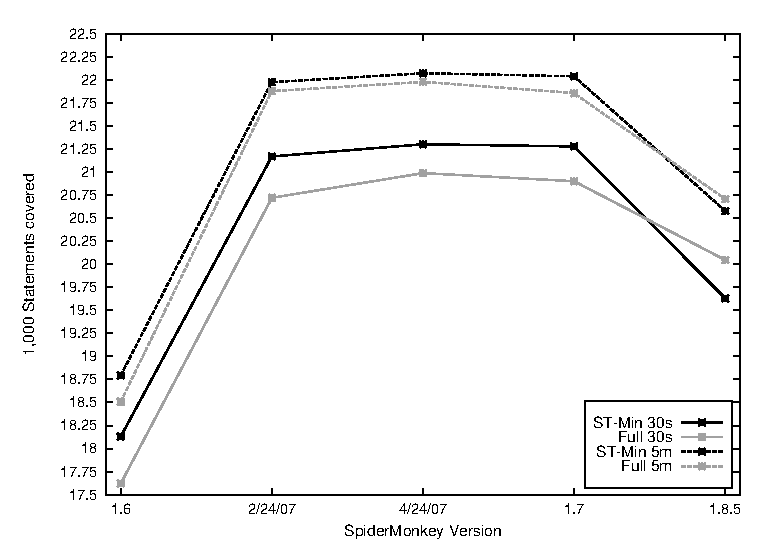
\includegraphics[width=\columnwidth]{scov}
  \caption{ST coverage for 30s and 5m quick tests across SpiderMonkey versions}
  \label{fig:scov}
\vspace{-0.2in}
\end{figure}


Table \ref{tab:unlimited} provides information on the base test suites
across the five versions of SpiderMonkey studied.  Tables
\ref{tab:run30s} and \ref{tab:run5m} show how each proposed quick test
approach performed on each version, for 30 second and 5 minute test
budgets, respectively.  All experiments with nondeterminstic results
(random or time-based selection) were repeated 30 times, and all
comparisons between values for different methods are statistically
significant under a two-tailed U-test, with $p$-values $<$ (often much less
than) 0.01.  The best results for each suite attribute, SpiderMonkey
version, and test budget combination are shown in bold (ties are only
shown in bold if some approaches did not perform as well as the best
methods).  Results for absolute coverage prioritization are omitted
from the table in the interest of space, as $\Delta$ prioritization
always performed better, and absolute often performed worse than
random selection.

The results are fairly striking.  First, a purely failure-based quick
test such as was used at NASA ({\bf DD-Min}) produces very poor code
coverage (e.g., covering almost 100 fewer \emph{functions} than the
original suite, and over 300 fewer branches).  It also loses fault
detection power rapidly, only finding $\sim$7 distinct faults on the
next version of the code base, while suites based on all tests can
detect $\sim$20-$\sim$36 faults.  Given its extremely short runtime,
retaining such a suite as a pure regression may be useful, but it
cannot be expected to work as a good quick test.  Second, the suites
greedily minimized by statement coverage ({\bf GE-ST(Full)} and {\bf
GE-ST(ST-Min)}) are very quick, and potentially useful, but lose a
large amount of branch coverage and do not provide enough tests to
fill a 5 minute quick test.  The benefits of suite minimization by
statement coverage (or branch coverage) were represented in the 30
second and 5 minute budget experiments by the $\Delta$ prioritizations,
which produce the same results, with the exception that for short
budgets tests included because they uniquely cover some entity are
less likely to be included than with random sampling of the minimized
suites.

The most important total suite result is that the cause reduced {\bf
ST-Min} suite retains (or improves!) many properties of the {\bf Full}
suite that are \emph{not} guaranteed to be preserved by our modified
\emph{ddmin} algorithm.  For version 1.6, only 5 branches are
``lost'', and (most strikingly) the number of failing test cases is
\emph{unchanged}.  Most surprisingly, the estimated distinct fault
detection is \emph{improved}: it has grown from $\sim$22 faults to
$\sim$43 faults.  This improvement is highly statistically
significant: dividing the test population into 30 equal-sized randomly
selected test suites for both full and minimized tests we find that
the average minimized suite detects 11.83 distinct faults on average,
while the average full suite only detects 7.6 faults, with $p$-value
of $5.2 \dot 10^{-10}$ under a two-tailed U-test.  It is difficult to
believe that any bias in the fault estimation method produces this
strong an effect.  Our best hypothesis as to the cause of the
remarkable failure preservation level is that \emph{ddmin} tends to
preserve failure because failing test cases have unusually \emph{low}
coverage in many cases.  Since the \emph{ddmin} algorithm attempts to
minimize test size, this naturally forces it to attempt to produce
reduced tests that also fail; moreover, some failures execute internal
error handling code (many do not, however --- the numerous test cases
violating \texttt{jsfunfuzz} semantic checks, for example).  The
apparent increased diversity of faults, however, is surprising and
unusual, and suggests that the use of \emph{ddmin} as a test
mutation-based fuzzing tool might be a promising area for future
research.  In retrospect, it is obvious that \emph{ddmin} takes as
input a test case and generated a large number of related, but
distinct, new test cases --- it is, itself, a test case generation
algorithm.  It seems safe to say that the new suite is essentially as
good at detecting faults and covering code, with much better runtime
(and therefore better test efficiency \cite{gupta-jalote-sttt06}).

Moreover, for versions of SpiderMonkey up to four months (at least)
after the creation of quick test candidate suites, not only is {\bf
ST-Min} a better source for quick tests than the {\bf Full} suite, it
is better to perform \emph{random selection on the reduced suite than
to use coverage-based prioritization on the full suite}.  This holds
despite the fact that $\Delta$-coverage based prioritization usually
improved coverage for 30 second test budgets, and often improved it
for 5 minute budgets.  The improvement on prioritization is present
even for the 1.7 release version, with the exception that $\Delta$-ST
prioritization of the {\bf Full} suite is better for fault detection
than random selection from {\bf ST-Min}.  It is only with the 1.8.5
release, over four years later, that the reduced suite is clearly
generally less effective.  Even for 1.8.5, however, $\Delta$BR
prioritization of {\bf ST-Min} produces the best function coverage of
any method.  In reality, it is highly unlikely that developers would
not have a chance to produce a better baseline on more similar code in
a four year period (or, for that matter, in any two-month period).
Figure \ref{fig:scov} graphically exhibits the raw differences in
statement coverage for the suites as quick tests, ignoring the effects
of prioritization.

The power of coverage-based cause reduction can also be seen by
comparing ``equivalent'' rows for any version and budget: results for
each version are split so that {\bf Full} results are the first five
rows and the corresponding prioritization the for {\bf ST-Min} tests
are the next five rows.  For the first three versions tested, it is
almost always the case that for every measure, the reduced suite value
is better than the corresponding full suite value.  For 30s budgets
this comparison even holds true for the 1.7 version, nearly a year
later.  Moving from 1.6 to 1.7 involves over 1,000 developer commits
and the addition of 10,000+ new lines of code (a 12.5\% increase).

It is difficult to generalize from one subject, but based on the
SpiderMonkey results, we believe that a good initial quick test
strategy to try for other projects would be to combine cause reduction
by statement coverage with test case prioritization by either $\Delta$
statement or branch coverage.  In fact, our limitation of quick tests
to very small budgets may not be critical here.  The 


\section{YAFFS 2.0 Flash File System Case Study}

\begin{table*}[t]
\caption{YAFFS2 Results}
\centering
\label{tab:yaffs}
\begin{tabular}{|c||c|c|c|c|c|c|c|c}
\hline
Suite & \#Tests & Time(s) & ST & BR & FN & MUT & Notes \\
\hline
\hline
Full & 4,240 & 729.032 & 4,049 & 1,925 & 332 & 616 & Kills 11 mutants not killed by {\bf ST-Min} \\
\hline
ST-Min & 4,240 & 402.497 & 4,049 & 1,924 & 332 & 611 & Kills 6 mutants not killed by {\bf Full} \\ 
\hline
\hline
\hline
Full 30s & 175.9 & 30.0 & 4,009.6 & 1,849.9 & 332.0 & 570.0 & \\
\hline
Full $\Delta$ST 30s & 373.0 & 30.0 & {\bf 4,049.0} & 1,918.0 & 332.0 & 594.0 & \\
\hline
Full $\Delta$BR 30s & 113.0 & 30.0 & 4,031.0 & 1,900.0 & 332.0 & 593.0 & \\
\hline
\hline
ST-Min 30s & 315.1 & 30.0 & 4,018.9 & 1,854.0 & 332.0 & 560.5 & \\
\hline
ST-Min $\Delta$ST 30s & 514.0 & 30.0 & {\bf 4,049.0} & 1,912.0 & 332.0 & {\bf 601.0} & \\
\hline
ST-Min $\Delta$BR 30s & 550.0 & 30.0 & {\bf 4,049.0} & {\bf 1,924.0} & 332.0 & 575.0 & \\
\hline
\hline
\hline
Full 5m & 1,739.9 & 300.0 & 4,043.2 & 1,910.6 & 332.0 & {\bf 608.8} & \\
\hline
Full $\Delta$ST 5m & 2,027.0 & 300.0 & {\bf 4,049.0} & 1,921.0 & 332.0 & 601.0 & \\
\hline
Full $\Delta$BR 5m & 2,046.0 & 300.0 & {\bf 4,049.0} & {\bf 1,925.0} & 332.0 & 604.0 & \\
\hline
\hline
ST-Min 5m & 3,156.6 & 300.0 & 4,047.0 & 1,918.9 & 332.0 & 607.1 & \\
\hline 
ST-Min $\Delta$ST 5m & 3,346.0 & 300.0 & {\bf 4,049.0} & 1,924.0 & 332.0 & 601.0 & \\
\hline
ST-Min $\Delta$BR 5m & 3,330.0 & 300.0 & {\bf 4,049.0} & 1,924.0 & 332.0 & 605.0 & \\
\hline
\end{tabular}
\end{table*}

YAFFS2~\cite{yaffs2} is a popular open-source NAND flash file system
for embedded use; it was the default image format for early versions
of the Android operating system.  Lacking a large set of real faults
in YAFFS2, we applied mutation testing to check our claim that cause
reduction not only preserves source code coverage, but tends to
preserve fault detection and other useful properties of randomly
generated test cases. The evaluation used 1,992 mutants, randomly
sampled from the space of all 15,246 valid YAFFS2 mutants, using the C
program mutation approach (and software) shown to provide a good proxy
for fault detection by Andrews et~al.~\cite{mutant}.  Random sampling
of mutants has been shown to provide useful results in cases where
full evaluation is not feasible, and the sample rate of 13.1\% exceeds
the 10\% threshold suggested in the literature~\cite{MutRand}.
Sampled mutants were not guaranteed to be killable by the API calls
and emulation mode tested.  Table \ref{tab:yaffs} shows how suites for
YAFFS2 compared, omitting $|$ST$|$ and $|$BR$|$ in the interest of
space; these performed poorly for coverage, though maximized mutant
kills to 611/610 for both base suites at 5 minutes.  The poorer
performance of {\bf ST-Min} at 5 minutes here is probably because
runtime reduction for YAFFS2 was not as high as with SpiderMonkey
tests (1/2 reduction vs. 3/4), due to a smaller change in test size:
the average length of original test cases was 1,004 API calls, while
reduced tests averaged 213.2 calls.  Basic retention of desirable
aspects of {\bf Full} was, however, excellent: only one branch was
``lost'', function coverage was perfectly retained, and 99.1\% as many
mutants were killed.  The reduced suite killed 6 mutants not killed by
the original suite.  While we do not know if mutant scores are good
indicators of the ability of a suite to find, e.g., subtle
optimization bugs in compilers or, mutant kills \emph{do} seem to be a
reliable method for estimating the ability of a suite to detect the
many of the shallow bugs a quick test aims to expose before code is
committed or subjected to more testing.  Even with lesser efficiency
gains, cause reduction plus $\Delta$ST is the best way to produce a 30
second quick test.

\section{GCC: The Potentially High Cost of Reduction}

Finally, we attempted to apply cause reduction to test cases produced
by Csmith \cite{csmith} using the GCC 4.3.0 compiler (released
3/5/2008), using C-Reduce \cite{CReduce} modified to attempt only
line-level reduction, since we hypothesized that reducing C programs
would be more expensive than reducing SpiderMonkey or YAFFS2 test
cases, which have a simpler structure.  Our hypothesis proved more
true than we had anticipated: after 6 days of execution (on a single
machine rather than a cluster), our reduction produced only 12 reduced
test cases!  The primary problem is twofold: first, each run of GCC
takes longer than the corresponding query for SpiderMonkey or YAFFS2
tests, due to the size and complexity of GCC (tests are covering 161K+
lines, rather than only about 20K as in SpiderMonkey) and the inherent
start up cost of compiling even a very small C program.  Second, the
test cases themselves are larger --- an average of 2,222 reduction
units (lines) vs. about 1,000 for SpiderMonkey and YAFFS --- and
reduction fails more often than with the other subjects.

While 12 reduced test cases do not make for a particularly useful data
set, the statistics for these instances did support the belief that
reduction with respect to statement coverage preserves interesting
properties.  First, the 12 test cases selected all crashed GCC 4.30
(with 5 distinct faults, in this case confirmed and examined by hand);
after reduction, the test cases were reduced in size by an average of
50\%, and all tests still crashed GCC 4.3.0 with the same faults.  For
GCC 4.4.0 (released 4/21/2009), no test cases in either suite caused
the compiler to fail, and the reduced tests actually covered 419
\emph{more} lines of code when compiled. Turning to branch coverage,
an even more suprising result appears: the minimized tests cover an
additional 1,034 branches on GCC 4.3.0 and an additional 297 on 4.4.0.
Function coverage is also \emph{improved} in the minimized suite for
4.4.0: 7,692 functions covered in the 12 minimized tests vs. only
7,664 for the original suite.  Unfortunately the most critical
measure, the gain in test efficiency, was marginal: for GCC 4.3.0, the
total compilation time was 3.23 seconds for the reduced suite vs. 3.53
seconds for the original suite, though this improved to 6.35s vs 8.78s
when compiling with GCC 4.4.0. Even a 50\% size reduction does not
produce much runtime improvement, due to the high cost of starting
GCC.

\section{Threats to Validity}

First, we caution that cause reduction by coverage is intended to be
used on the highly redundant, inefficient tests produced by aggressive
random testing.  While random testing is sometimes highly effective
for finding subtle flaws in software systems, and essential to
security-testing, by its nature it produces test cases open to extreme
reduction.  It is likely that human-produced test cases (or test cases
from directed testing that aims to produce short tests) would be not
reduce well enough to make the effort worthwhile.  The quick test
problem is formulated specifically for random testing, though we
suspect that the same arguments also hold for model checking traces
produced by SAT or depth-first-search, which also tend to be long and
redundant.

The primary threat to validity is that experimental results are based
on one large case study on a large code base over time, one mutation
analysis of a smaller but also important and widely used program, and
a few indicative tests on a very large system, the GCC compiler.
